\chapter{Low temperature environments}
\section{Introduction}
\begin{itemize}
    \item Low temperature: \SI{-273}{\degree C}, \SI{-150}{\degree C}
    \item Mechanical challenges - rapid heating / increasing gas pressure
          \begin{itemize}
              \item Failure / fatigue
          \end{itemize}
    \item Most low temperature - rise at atmospheric pressure
          \begin{itemize}
              \item Small volumes
          \end{itemize}
    \item Through design - challenge becomes managing the thermal component not the mechanical
    \item Health \& Safety - dense / cold gas moves quickly and can suffocate people
\end{itemize}
\begin{table}[H]
    \centering
    \begin{tabular}{@{}ll@{}}
        \toprule
        \textbf{Gas} & \textbf{Freezing temperature}      \\
        \midrule
        \ce{CO2}     & \SI{-78.5}{\degree C} (sublimates) \\
        Nitrogen     & \SI{-196}{\degree C}               \\
        LNG          & \SI{-161.5}{\degree C}             \\
        \bottomrule
    \end{tabular}
    \caption{Freezing temperatures of various gases.}
\end{table}
The energy density of LNG is comparable to propane and ethanol but is only 60 percent that of diesel and 70 percent that of gasoline.
\begin{figure}[H]
    \centering
    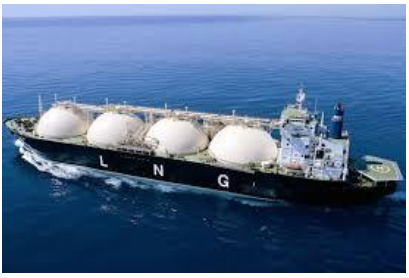
\includegraphics[width = 0.5 \textwidth]{img/figure56.png}
    \caption{LNG carrier.}
\end{figure}
An LNG carrier is a tank ship designed for transporting liquefied natural gas. At the end of 2016, the global LNG shipping fleet consisted of 439 vessels. Majority of ships have a capacity of \SI{120000}{}-\SI{140000}{\meter\cubed}.
\begin{table}[H]
    \centering
    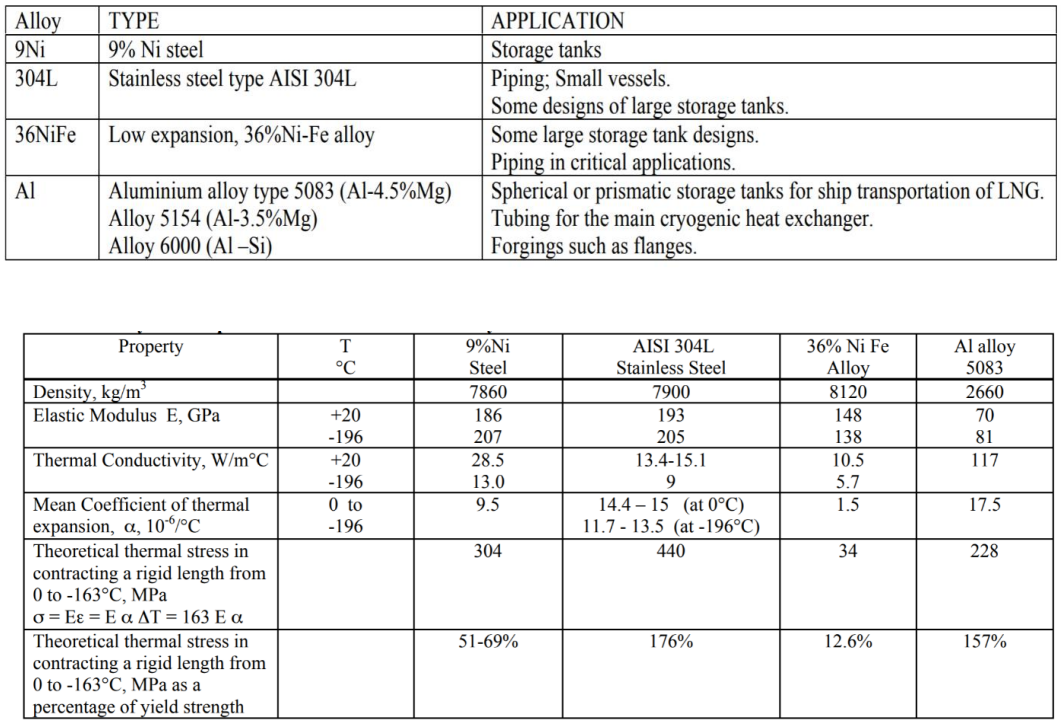
\includegraphics[width = \textwidth]{img/figure57.png}
    \caption{Tables to show material properties of storage tanks.}
\end{table}
\begin{table}[H]
    \centering
    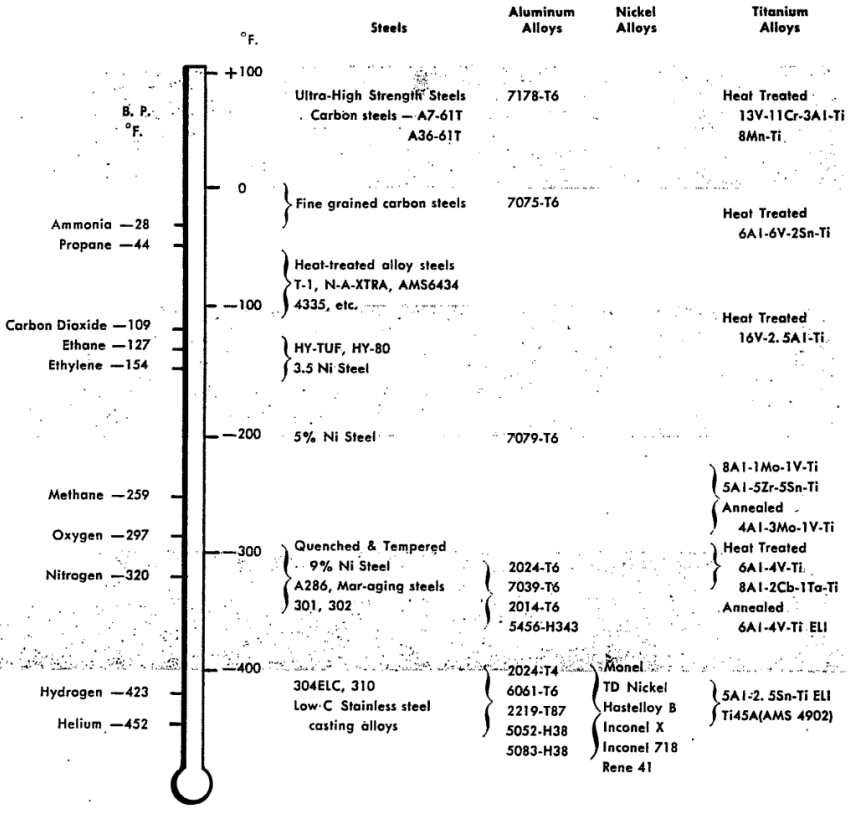
\includegraphics[width = \textwidth]{img/figure58.png}
    \caption{Table to show materials used to store different low temperature materials.}
\end{table}
\section{Engineering applications}
\subsection{LNG - liquefied natural gas}
Methane, \ce{CH4} (with some ethane). 1/6000$^{\textrm{th}}$ the volume of natural gas in the gaseous state (at standard condition for temperature and pressure). It is odourless, colourless, non-toxic and non-corrosive. Hazards include flammability after vaporisation into a gaseous state, freezing and asphyxia. The liquefaction process involves removal of certain components, such as dust, acid gases, helium, water and heavy hydrocarbons, which could cause difficulty downstream. The natural gas is then condensed into a liquid at close to atmospheric pressure by cooling it to approximately \SI{-162}{\degree C}. Maximum transport pressure is set at around \SI{25}{\kilo\pascal}.
\subsection{Cryogenic transport}
Transfer lines are a form of cryostat. Used to transport cryogenic fluids between cryogenic devices. Simplest form is a vacuum jacketed pipe connecting two flasks. Heat is absorbed by the liquid (nitrogen) and as the pipe gets longer, more heating occurs and more vapour generated (which is lost). Higher pressure differential, more heating occurs. The most important design elements are:
\begin{itemize}
    \item Geometry
    \item Mass flow rate
    \item Temperature and pressure change
    \item Cryogenic fluid
    \item Mechanical properties of the materials
\end{itemize}
\section{Thermal bowing}
\begin{figure}[H]
    \centering
    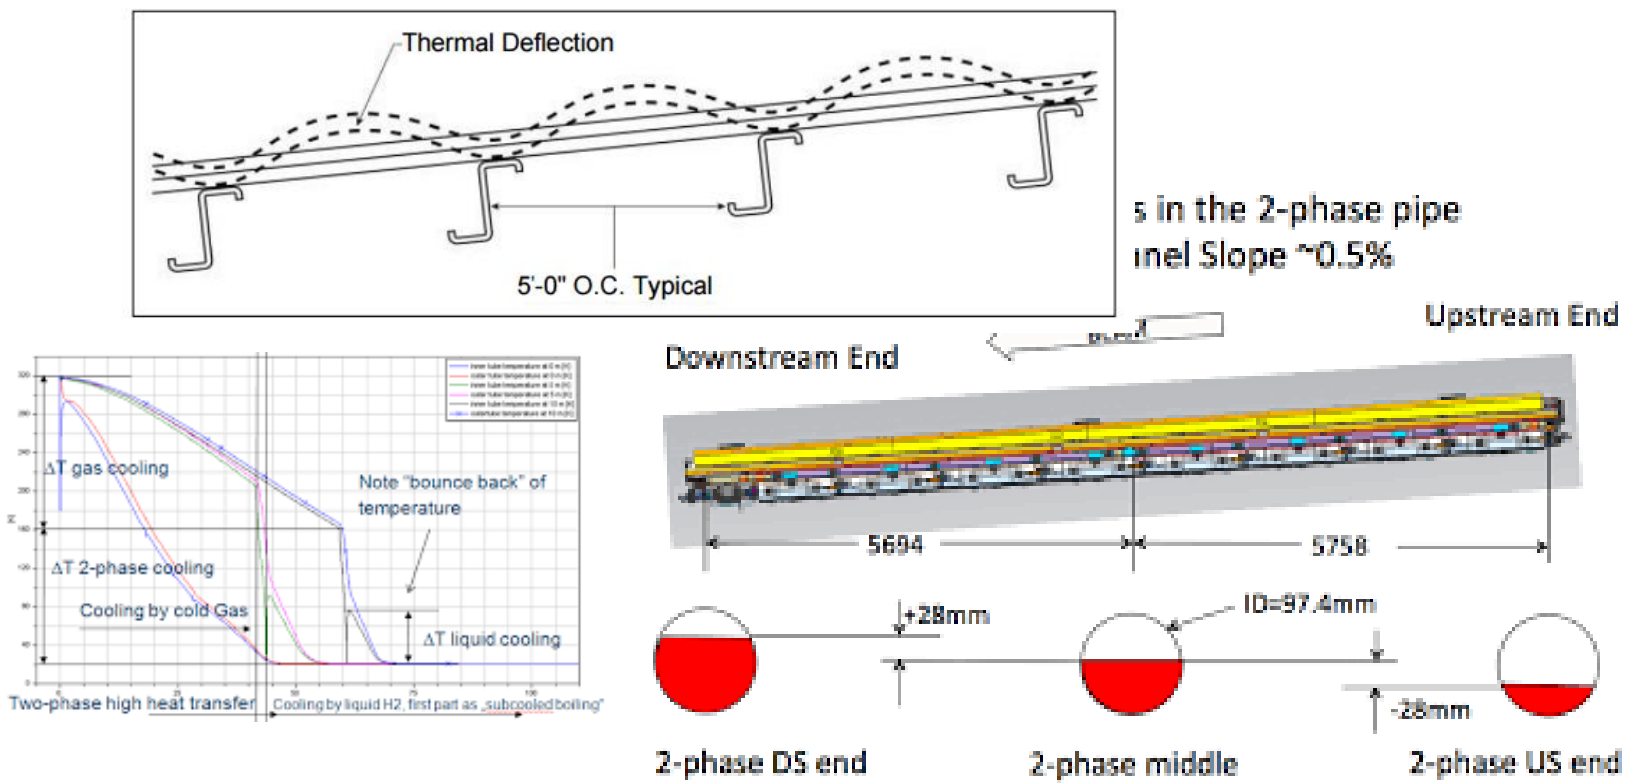
\includegraphics[width = \textwidth]{img/figure59.png}
    \caption{Thermal bowing.}
\end{figure}
\subsubsection{Laterial variation of temperature}
Thermal bowing occurs due to two processes:
\begin{enumerate}
    \item Restrained thermal expansion
    \item Temperature gradient across pipe
\end{enumerate}
Assuming no mean temperature increase:
\begin{equation}
    \Delta T = 0
\end{equation}
\begin{figure}[H]
    \centering
    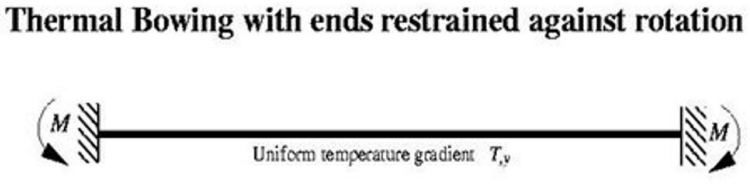
\includegraphics[width = 0.6\textwidth]{img/figure60.png}
    \caption{Fixed end beam subjected to a uniform thermal gradient.}
\end{figure}
Uniform moment over the length:
\begin{equation}
    M = EI \phi = EI\alpha T_{,y}
\end{equation}
\begin{figure}[H]
    \centering
    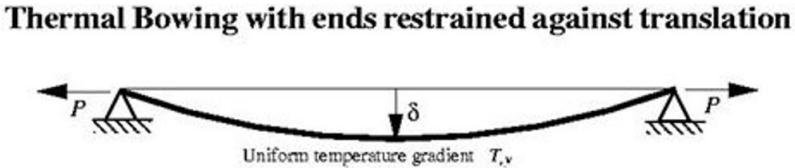
\includegraphics[width = 0.6\textwidth]{img/figure61.png}
    \caption{Laterally restrained beam subjected to a uniform thermal gradient.}
\end{figure}
A tensile force $P$ will be generated causing a tensile $P-\delta$ moment $Py$ over the length of the beam,
\begin{equation}
    \frac{\dif^2 y}{\dif x^2} = \phi + \frac{Py}{EI}
\end{equation}
or
\begin{equation}
    \frac{\dif^2 y}{\dif x^2} - k^2 y = \phi
\end{equation}
where,
\begin{equation}
    K = \sqrt{\frac{P}{EI}}
\end{equation}
The solution of this equation is,
\begin{equation}
    y\left(x\right) = -\frac{\phi}{k^2}\left(\frac{\cosh\left(kl\right) - 1}{\sinh\left(kl\right)}\sinh\left(kx\right)\cosh\left(kx\right)+1\right)
\end{equation}
\subsubsection{Derivation}
The derivation starts with the point that the displacement is:
\begin{equation}
    u = f\left(x\right) + yf_1\left(x\right) + zf_2\left(x\right)
\end{equation}
The longitudinal strain is
\begin{equation}
    \epsilon_{xx} = \frac{\partial u}{\partial x} = f'\left(x\right) + yf_1'\left(x\right) + zf_2'\left(x\right)
\end{equation}
The stress field is
\begin{equation}
    \sigma_{xx} = E \left(\epsilon_{xx} - \alpha T\right)
\end{equation}
The equilibrium constraints are
\begin{align}
    \int \sigma \dif A   & = 0 \\
    \int \sigma y \dif A & = 0 \\
    \int \sigma z \dif A & = 0
\end{align}
The geometrical constraint is
\begin{equation}
    \int y \dif A = \int z \dif A = 0
\end{equation}
Cross-pipe variation of temperature:
\begin{equation}
    \sigma_{xx} = -\alpha E\left(T - \bar{T}\right) + \frac{I_yM_{Tz}-I_{yx}M_{Ty}}{I_yI_z-I^2_{yz}}y + \frac{I_yM_{Tz}-I_{yx}M_{Ty}}{I_yI_z-I^2_{yz}}z
\end{equation}
where
\begin{align}
    I_z    & = \int y^2 \dif A        \\
    I_y    & = \int z^2 \dif A        \\
    I_{yz} & = \int yz \dif A         \\
    M_{Ty} & = \int \alpha ETz \dif A \\
    M_{Tz} & = \int \alpha ETy \dif A
\end{align}
For a pipe
\begin{equation}
    \sigma_{xx} = -\alpha E \left(T - \bar{T}\right) + \frac{M_{Tz}}{I_y}y
\end{equation}
For the lateral displacement
\begin{gather}
    \frac{\dif^2 v}{\dif x^2} = - \frac{M_{Tz}}{EI_z}\\
    \frac{\dif}{\dif x^2}\left(EI_z\frac{\dif^2 v}{\dif x^2}\right) + \frac{\dif^2 M_{Tz}}{\dif x^2} = F
\end{gather}
\begin{figure}[H]
    \centering
    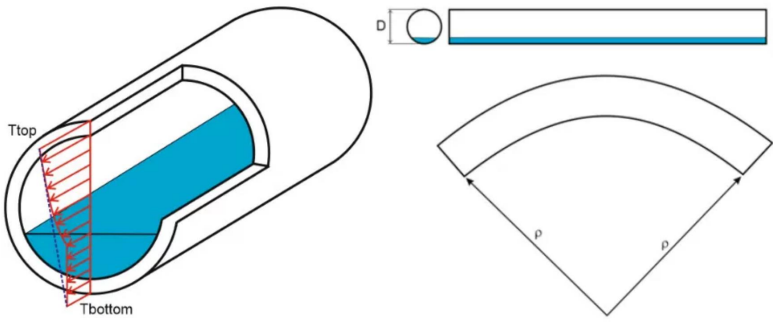
\includegraphics[width = 0.6\textwidth]{img/figure62.png}
    \caption{Cross-section of pipe.}
\end{figure}